\section{Discussion of our results}
\label{sec:discrepancies}
As we have seen in section~\ref{sec:results}, we have not obtained the 
expected results from our simulations in all cases. In this section we discuss 
possible reasons for this discrepancy between the expected and actual results, 
and some possible changes that we believe will fix these discrepancies.

The section is divided into two parts: in the first we discuss possible errors 
related to our implementation of the simulation, and in the second part we 
discuss changes to the model that might fix some of the discrepancies.

\subsection{Our implementation of the simulations}
\label{sec:random-errors}
We have attempted to implement the simulation of the model that is as close to 
the description of the model as possible. However, as we have seen in 
section~\ref{sec:model-to-simulation}, there has been some areas where we have 
had to fill in some details that have not been explained in the articles 
describing the model. Indeed, in the formulation of the model itself, we have 
been forced to add features from different articles because the description in 
the original article was insufficient. It is possible that some of these 
necessary additions have been done differently than seen in the simulations 
performed by the authors of the original articles, and that this contributes 
to the discrepancies between the their results and ours.

Of course we cannot completely rule out errors in our implementation either; 
while we do not believe any obvious errors exist, we do not have anything to 
compare it with that has the same level of detail. The only thing we have to 
compare our implementation with, is the code underlying \cite{helbing00}, 
which the authors have published on their website. However, this code is quite 
inscrutable, so it would require considerable effort to analyse it and compare 
it with our own. A cursory glance indicates that there are features in it that 
we do not have in our implementation; whether these are vital or not we cannot 
say.

A final thing that relates to the implementation of the simulation is the 
setting of parameters and initial conditions. The values for the different 
parameters have not always been given along with their description in the 
articles describing the model. This means we have had to find the values 
elsewhere, and this mixing of parameters from different sources might also be 
a source of errors. Finally, the use of random values for initial conditions 
(in the setting of pedestrian starting positions, size and initial desired 
speed) is a possible source of error. While we set a mean value and a standard 
deviation on the generated values, in some cases extremely high or low values 
are generated. An example of this is seen in figure~\ref{fig:random-seed}, 
where one pedestrian starts out with a very low desired velocity, causing it 
to move extremely slowly. The long leaving time is then not caused by clogging 
of the exit, but simply by the delay from the time it takes the pedestrian to 
cross the distance between its starting point and the exit.

\begin{figure}[h]
    \centering
    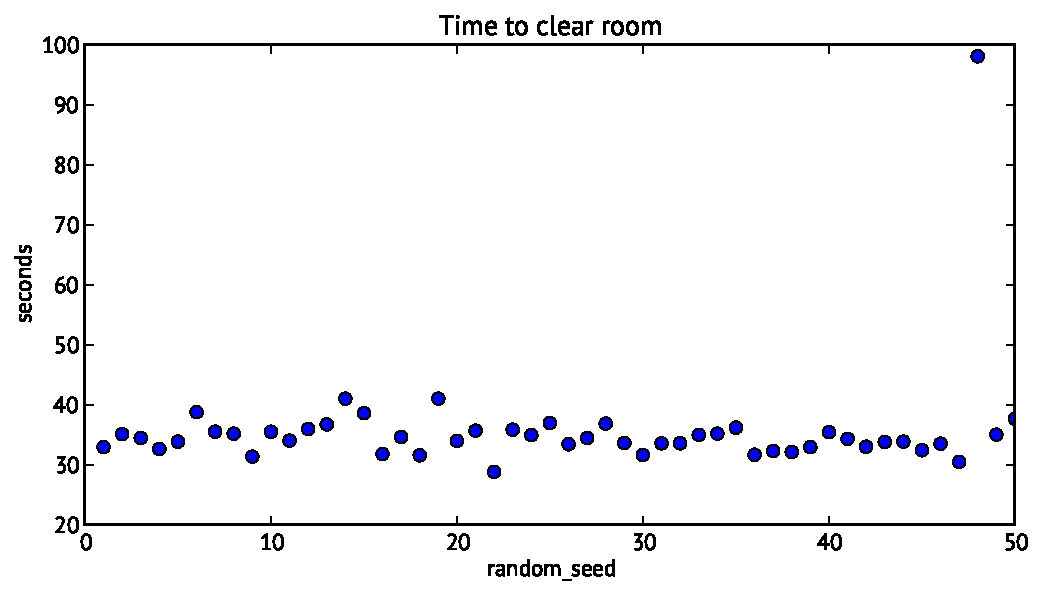
\includegraphics[width=0.8\textwidth]{Figures/random-seed-variations.pdf}
    \caption[Leaving time for different random seeds]{Leaving time for 
    different random seeds. Results are dependent on random numbers; for a 
    seed value of 48 (top-right corner), one pedestrian starts out walking 
    very slowly impacting the total leaving time.}
    \label{fig:random-seed}
\end{figure}



\subsection{Clogging in narrow places}
The article \cite{self-org} claims that social force models are able to reproduce the clogging phenomena which arises when a large number of pedestrians try to pass a narrow passage. This phenomena is also know as the "faster is slower phenomena". Through our simulation this phenomena has not occurred.



\subsection{Pedestrians overlapping and walking through walls}
A problem we encountered during the simulation was pedestrians walking through walls and/or pedestrians overlapping. Both these scenarios are illustrated in figure \ref{fig:problemSenario}. This could be caused by the size of the time step see section \ref{constants}, but the time step can not always correct this problem.

A person can have a resulting force which points towards the wall even as the distance to the wall approaches zero. This problem arise when pedestrians are moving fast and are unable to stop in time and occurs because the model do not take into account how fast pedestrians are approaching walls or other pedestrians.

In other words, a pedestrian running towards a wall will decelerate at the same rate as a person walking towards the wall. One could argue that this is unrealistic behaviour because, the person running should start decelerating sooner than the person walking. A person which has a force towards the wall which exceed the force he feels from the wall, then he will always go through the wall. This phenomena is off course not dependent on the time step, since even with a infinity small time step this could occur. One way of elimination this problem is by making the force a pedestrian feel depend not only on the distance to the obstacle but also depend on the current speed towards this obstacle. Such a feature has been documented to improve the predictions of the model\cite{ABconstant}.
\begin{figure}
\centering
\subfloat[Overlapping occurs when speeds get to high in this case $2.50m/s$ which prevents pedestrians from stopping in time.]{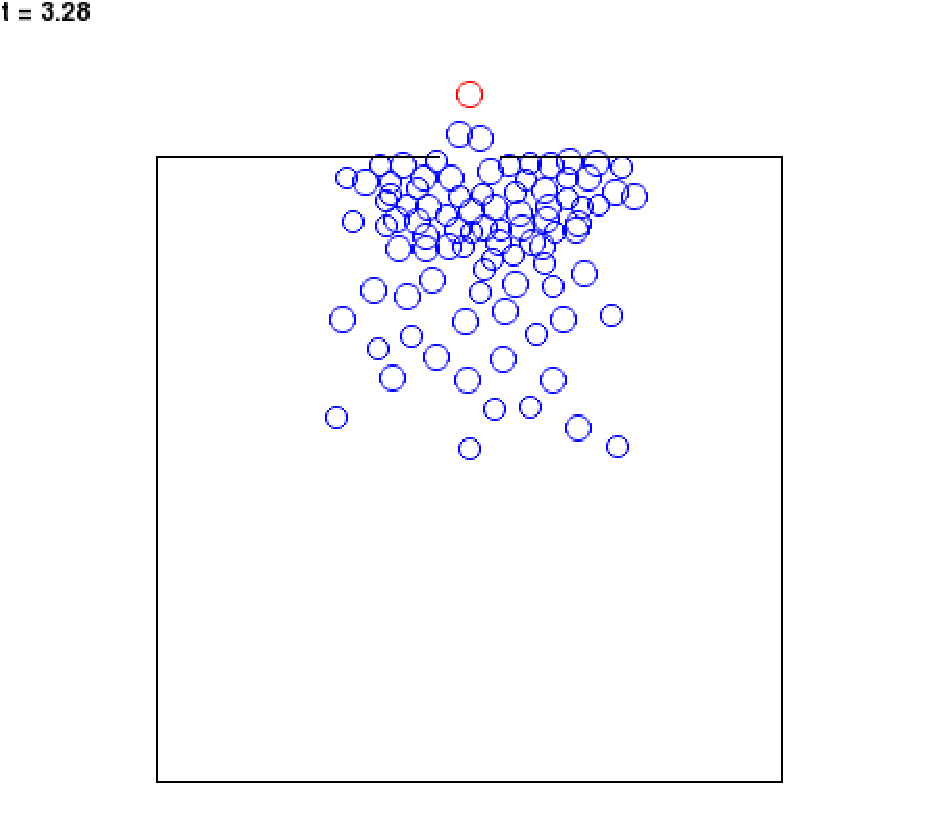
\includegraphics[scale=0.5]{Figures/squareRoomOverlapping}}
\subfloat[A single pedestrian escapes through the wall due to a initial speed of $3.50m/s$]{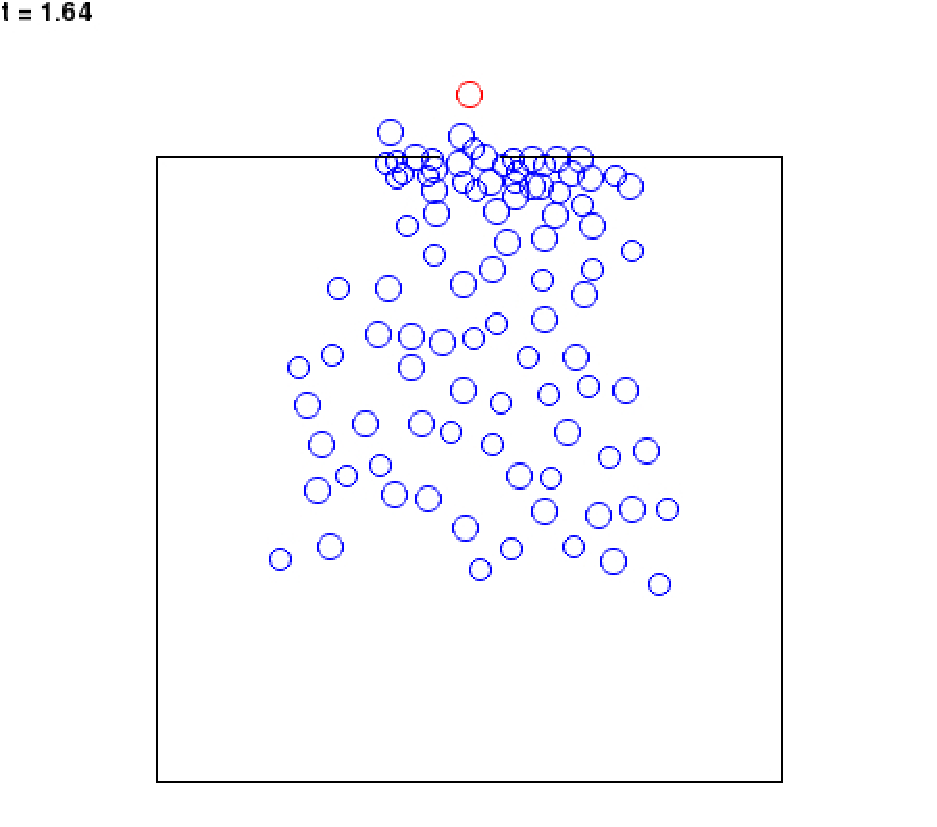
\includegraphics[scale=0.5]{Figures/squareRoomThrowWall}}
\caption{These pictures was produced with the following values: $A=2.2$, $B=0.2$, $U=2.0$, Pedestrian number=$100$, $\lambda=0.1$, $v^{max}_0=1.3 \cdot v_0$, $\tau = 1.0$, $\triangle t = 0.01$, only the starting velocity was changed}
\label{fig:problemSenario}
\end{figure}
\subsection{Faster-is-slower effect}
The article \cite{self-org} claims that social force models are models which are capable of representing the faster-is-slower effect. In our simulations people leave the room faster and faster as we increase their max speed. The article 

\subsection{Tangential forces}
Here we discuss the idea of improving the model by improving tangential forces, that is, the force parallel to the surface of an object.
The tangential forces can be used as collision avoidance, so that pedestrians steer around obstacles or other pedestrians \cite{tang}.
This would be relevant when simulating an environment where, e. g., and is standing in the middle of a symmetrical room and the pedestrian's waypoint
is behind a big square pillar, with equal distance either way around, the pedestrian would get stuck in front of the pillar without the tangential forces,
since the forces acting on the pedestrian's motivation is cancelling each other out. 
In our case where two groups of pedestrians are crossing each other in a corridor, the tangential force would make the pedestrians to into account
the position of the pedestrians in front of them and steer around them.
The tangential forces can also improve the model so it can simulate pedestrians escaping a smoke filled room where we determine the visibility.
In this case of simulation the pedestrians would walk randomly around untill they find a wall, and follow the wall around due to the tangential force.
This would be a way of implementing way finding to the model.

Friction between pedestrians would also be possible to add to the model, since the tangential forces from other pedestrians would make it
harder for pedestrians to walk through a crowd. \cite{self-org} mention that friction is causing clogging in front of exits, since the people
get stuck in each other. In our simulation the pedestrians are not clogging as heavily as \cite{self-org} mention it can be.
The time it take for the pedestrian to leave a room in unrealistic low, and we think that implementing the friction by tangential forces
would make the simulation time more realistic.

\subsection{Freezing by heating effect}
According to \cite{self-org} the freezing by heating effect should arise when the max desired velocity of the pedestrians was raised.
That is that clogging should arise when raising the max velocity of the pedestrians, because more are ariving to the possible
clogging area, and thus have more trouble getting through the crowd. 
We tried to raise the max velocity, see figure \ref{fig:freezingbyheating1} and figure \ref{fig:freezingbyheating05}, but instead of observing the freezing by heating effect, we saw that the pedestrians
got through the corridor more easely, and that the density in the corridor was lower when the max velocity was high.
We think that there are more explations to this result. For the first the pedestrian $\alpha$'s force toward the target
is higher when $\alpha$'s velocity gets higher, and therefore he more easely pushes his way through the crowd. For the second
there are no friction between the pedestrians to slow $\alpha$ speed down, besides the social sphere.

\subsection{Comparison between the relaxation time $1,0$ and $0,5$}
It is seen that the density in the corridor is more steady when the relaxation time is set to $0.5$.
This is true for both max desired velocity tested.

\begin{figure}[h]
\centering
\subfloat[The figure show the density in corridor when the relaxation time is set to $1,0$]{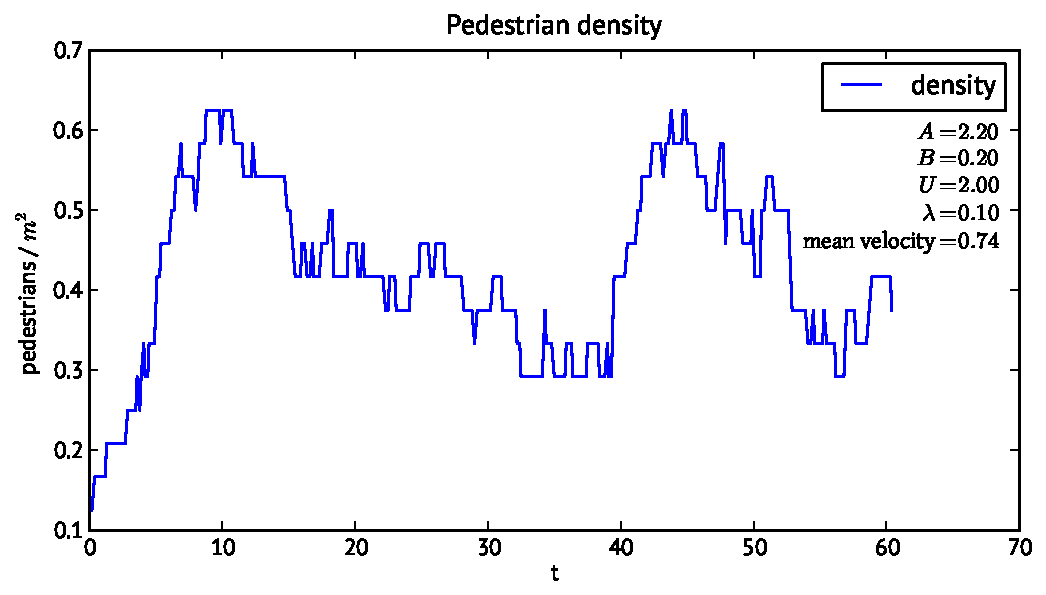
\includegraphics[scale=0.45]{Figures/dens_init_20.pdf}}
\subfloat[This figure shows the density in the corridor when the relaxation time is set to $0,5$]{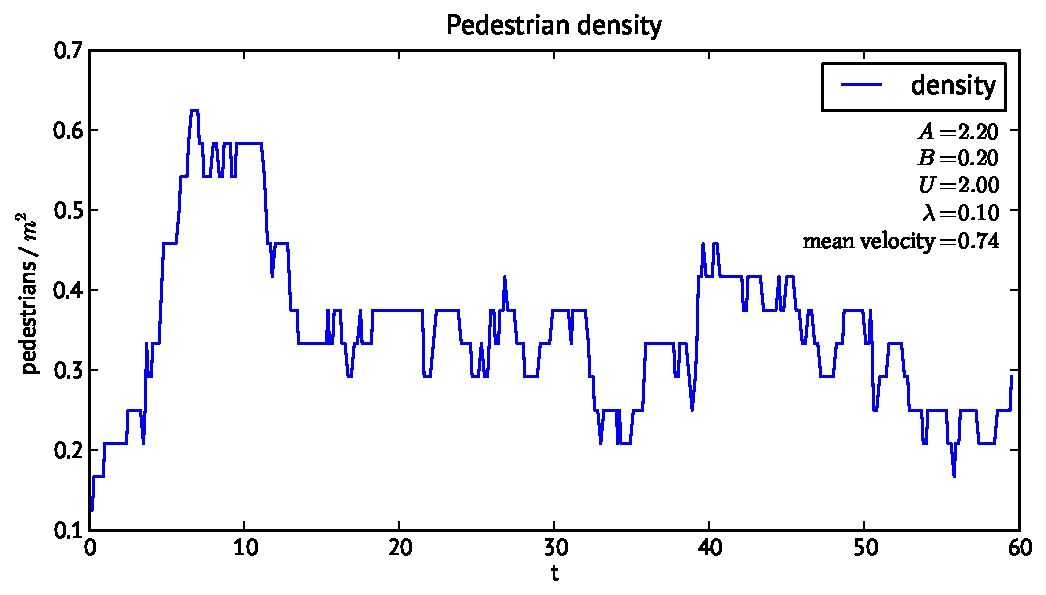
\includegraphics[scale=0.45]{Figures/dens_relax05_20.pdf}}
\caption{These figures show the difference of the density when changing the relaxation time of the model from $1$ to $0,5$.
It is seen the the density is more steady when the relaxtion time is $0,5$ instead of $1,0$}
\label{fig:comparison_of_timestep}
\end{figure}

A possible explanation of why the density is more steady through out the simulation when the relaxation time is $0,5$,
is that the pedestrians reacts faster to changes of their velocity. Thus when they bump into each other, they speed up
faster, and therefore avoid clogging up before more get in their path.

